%!TEX root = main.tex
\newpage
\chapter{StackLetter -- personalizovaný informačný bulletin pre Stack Exchange}

\textit{StackLetter} je systém pre vytváranie a rozosielanie personalizovaných informačných bulletinov vrámci platformy
Stack Exchange. Tento systém sme vyvinuli spoločne s kolegom Bc. Matúšom Salátom~\cite{Salat2018}. Celý systém sa skladá
z viacerých spolupracujúcich modulov, ktoré však boli vyvíjané samostatne a sú od seba navzájom nezávislé. Rozdelenie
systému na nezávislé moduly umožňuje rýchlejší vývoj, ako aj možnosť jednoduchého rozširovania systému v budúcnosti.
Architektonický prehľad celého systému znázorňuje obrázok~\ref{fig:architecutre-overview}. Ďalej v tejto práci popisujem
len mnou navrhnuté moduly.

\begin{figure}[H]\begin{center}
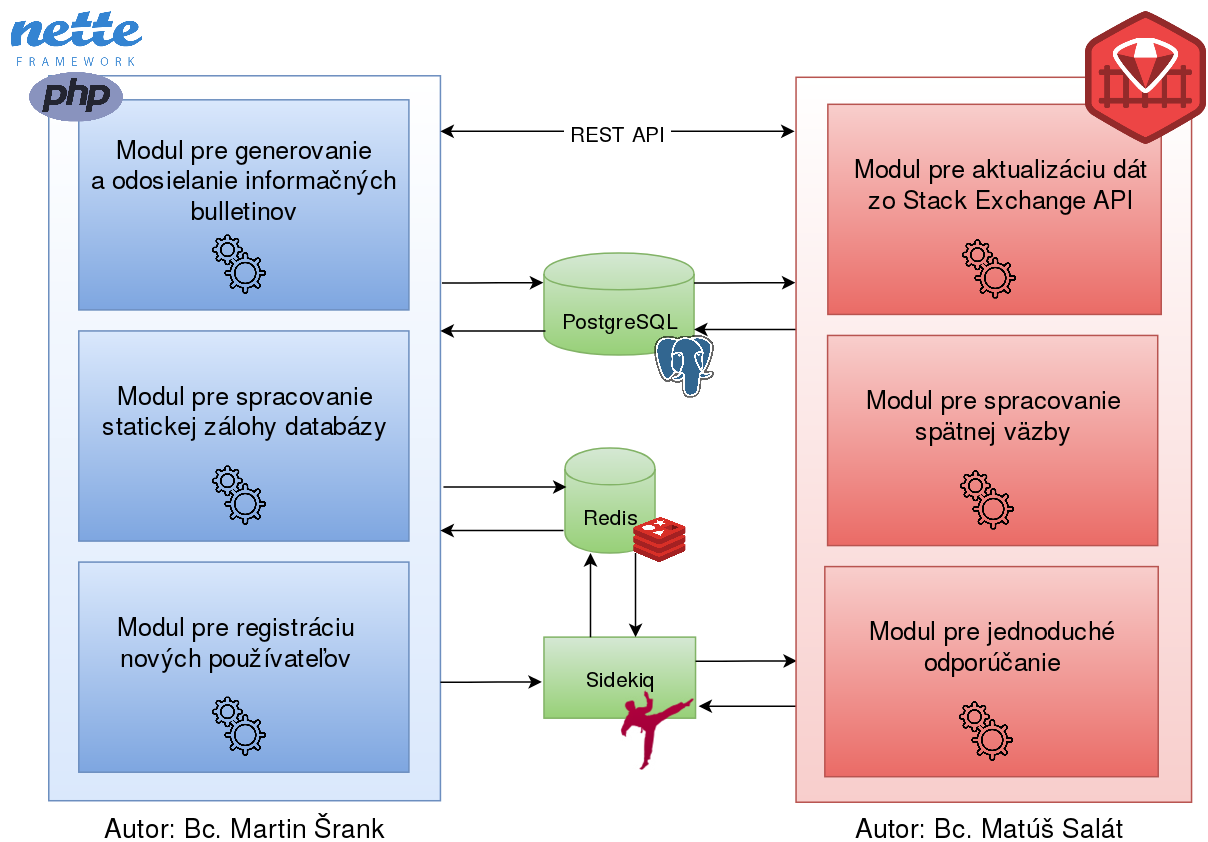
\includegraphics[scale=0.37]{architecture-overview}
\caption{Architektonický prehľad systému StackLetter. \label{fig:architecutre-overview}}\end{center}
\end{figure}

\section{Prehľad modulov}

\textbf{Modul pre registráciu nových používateľov}\\
Tento modul predstavuje používateľmi viditeľnú časť systému. Prostredníctvom webovej stránky systému
-- \url{www.stackletter.com} -- sa používatelia môžu prihlásiť k odoberaniu informačného bulletinu pre niektoré
z ponúkaných komunít platformy Stack Exchange, ako aj spravovať svoje nastavenia týkajúce sa odosielania informačných
bulletinov.\\
Používatelia sa prihlasujú prostredníctvom svojho Stack Exchange konta využitím protokolu OAuth.

\begin{figure}[H]\begin{center}
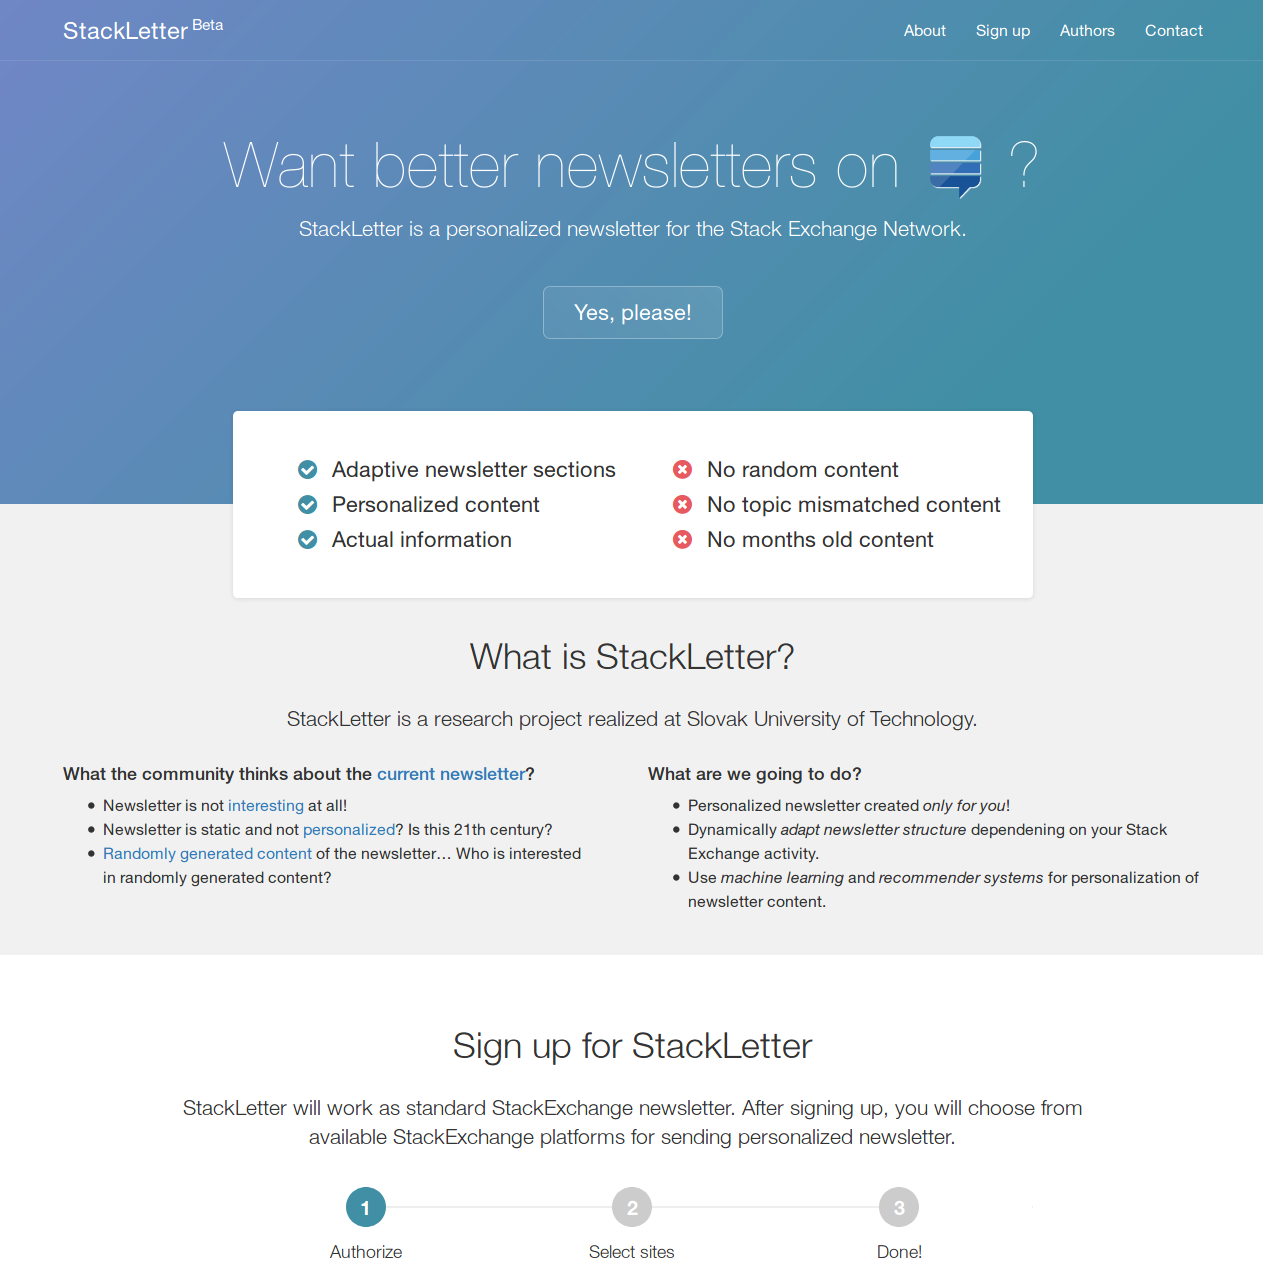
\includegraphics[scale=0.25]{stackletter-screenshot}
\caption{Snímka registračnej stránky StackLetter.com. \label{fig:stackletter.com}}\end{center}
\end{figure}

\textbf{Modul pre generovanie a odosielanie informačných bulletinov}\\
Tento modul je zodpovedný za samotné zostavovanie a odosielanie informačných bulletinov jednotlivým zaregistrovaným
používateľom. Prostredníctvom REST API komunikuje s modulmi pre zostavovanie odporúčaní a štruktúry informačných bulletinov
a na základe ich odpovedí vygeneruje naformátované informačné bulletiny, ktoré sú následne rozosielané prostredníctvom služby
SendGrid\footnote{\url{https://sendgrid.com}}.

\textbf{Modul pre spracovanie statickej zálohy databázy}\\
Modul bol navrhnutý a implementovaný za účelom rýchleho a efektívneho importovania počiatočných dát platformy Stack Exchange
dostupných vo forme XML exportu do našej internej reprezentácie v databáze PostgreSQL.

Podrobný technický a architektonický popis jednotlivých modulov sa nachádza
v prílohe~\ref{tech-doc} -- \textit{Technická dokumentácia systému StackLetter}.

\section{Použité technológie a služby}

\begin{my_itemize}
\item{Jednotlivé moduly zabezpečujúce infraštruktúru systému StackLetter sú implementované v~jazyku PHP\footnote{\url{https://php.net}}
verzie~7.1 s použitím MVC frameworku Nette~2.4\footnote{\url{https://nette.org}}.}
\item{Systém na ukladanie dát využíva relačný databázový systém PostgreSQL vo verzii 9.6 a vnútropamäťové dátové úložisko Redis
vo verzii 4.0.}
\item{Systém komunikuje s platformou Stack Exchange prostredníctvom Stack Exchange API v2.2 a~vykonáva autentifikáciu
používateľov prostredníctvom protokolu OAuth 2.0.}
\item{Na hromadné odosielanie informačných bulletinov používateľom prostredníctovm e-mailu je využitá služba SendGrid.}
\item{Modul implementujúci zostavovanie personalizovaných informačných bulletinov so zameraním na diverzitu bude implementovaný
v jazyku Python 3.6.}
\end{my_itemize}



\chapter{Experimentálne overenie}


\section{Návrh overenia metód}

Nami navrhnuté metódy personalizovaného odporúčania a diverzifikácie odporúčaného obsahu budeme overovať prostredníctvom
online nekontrolovaného experimentu spoločne s kolegom Matúšom Salátom~\cite{Salat2018} na používateľoch z komunity \textit{Stack Overflow} platformy Stack Exchange.

Tento online experiment bude mať formu pravidelne rozposielaného informačného bulletinu, na ktorého odoberanie sa budú
môcť prihlásiť všetci používatelia z tejto komunity.

Účinnosť zvolených metód diverzifikácie odporúčaní budeme vyhodnocovať prostredníctvom A/B testovania, pričom používateľov
rozdelíme na štyri skupiny:
\begin{my_enumerate}
    \item{Kontrolná skupina -- generický informačný bulletin bez odporúčania;}
    \item{Skupina A -- informačný bulletin s odporúčaním, bez diverzifikácie;}
    \item{Skupina B -- informačný bulletin s odporúčaním, metóda proporčnej diverzifikácie;}
    \item{Skupina C -- informačný bulletin s odporúčaním, metóda tématického vzorkovania;}
\end{my_enumerate}

Dôležitým predpokladom pre úspešnosť online experimentu bude získať dostatočnú reprezentatívnu vzorku používateľov
ochotných byť súčasťou experimentu. V~prípade, že by sa nám nepodarilo osloviť dostatočný počet používateľov, plánujeme
vykonať kontrolovaný offline experiment na vzorke archívnych dát.


\section{Metriky hodnotenia výsledkov}

Pre overovanie výsledkov experimentov budeme používať tieto metriky:

\textbf{Precision@N}\\
Presnosť (angl.~\emph{Precision}), alebo tiež \textit{pozitívna predikčná hodnota} je metrika reprezentujúca pomer relevantných
dokumentov z celkového zoznamu. Štandardne sa presnosť počíta ako pomer z celého zoznamu dokumentov, no v oblasti
odporúčania a vyhľadávania informácií je často vhodnejšou odvodená metrika \textit{Precision@N}, ktorá určuje, aká časť
z prvých N dokumentov v zozname je relevantná.
$$\mbox{Precision@N}=\frac{|\{\mbox{relevantne otazky v top-N}\}\cap\{\mbox{top-N odporucenych otazok}\}|}{|\{\mbox{top-N odporucenych otazok}\}|}$$

\textbf{nDCG}\\
\textit{Normalized Discounted Cumulative Gain} je metrika kvality ohodnocovania často používaná na meranie efektívnosti
odporúčania. DCG meria užitočnosť dokumentov na základe ich pozície vo výslednom zozname. Užitočnosť dokumentov sa akumuluje
od konca zoznamu, pričom najvyššiu užitočnosť majú dokumenty na začiatku zoznamu~\cite{Jrvelin2002}.

nDCG položky na pozícii $p$ v zozname odporúčaní je definované ako:

$$\mathrm{nDCG_{p}} = \frac{DCG_{p}}{IDCG_{p}}$$
$$\mathrm{DCG_{p}} = \sum_{i=1}^{p} \frac{ 2^{rel_{i}} - 1 }{ \log_{2}(i+1)}$$
$$\mathrm{IDCG_{p}} = \sum_{i=1}^{|REL|} \frac{ 2^{rel_{i}} - 1 }{ \log_{2}(i+1)}$$
\begin{adjustwidth}{1cm}{1cm}
$rel_i$ -- relevancia $i$-tej položky v zozname odporúčaní.\\
$|REL|$ -- zoznam $p$ relevantných položiek zo zoznamu odporúčaní usporiadaných podľa relevancie.
\end{adjustwidth}

\textbf{CTR}\\
Miera preklikov (angl.~\emph{Click-through Rate}) je metrika často využívaná v spojitosti s informačnými bulletinmi.
Táto metrika vyjadruje počet úspešných kliknutí na odkaz v informačnom bulletine.

Okrem CTR plánujeme v súvislosti s interakciou používateľa s informačným bulletinom merať aj počet impresií,
teda zobrazení informačného bulletinu, ako aj počet konverzií, teda podiel prípadov, kedy kliknutie na niektorú z otázok
v informačnom bulletine viedlo k aktivite používateľa na tejto otázke -- či už označenie za obľúbenú,
odpovedanie alebo pridanie komentáru. Ďalej tiež plánujeme merať počet odhlásení z informačného bulletinu.
